\documentclass{article}
\usepackage[T1]{fontenc}
\usepackage{lmodern}
\usepackage{graphicx}
\usepackage{amsmath,amssymb}
\usepackage[a4paper,margin=2cm]{geometry}
\usepackage[absolute,overlay]{textpos}
\setlength{\TPHorizModule}{1mm}
\setlength{\TPVertModule}{1mm}
\usepackage[indonesian]{babel}
\usepackage{hyperref}
\setlength{\emergencystretch}{2em}
% unit: Halaman 14

\begin{document}

% === Halaman 14 (llm) ===

% (tidak ada teks dari model)

% deskripsi: Screenshot cuplikan kode program bahasa C untuk implementasi algoritma enkripsi Rijndael (AES).
% bbox normalisasi: [0.1100, 0.4000, 0.8410, 0.9110]
\begin{textblock*}{153.51mm}(23.10mm,118.80mm)
\noindent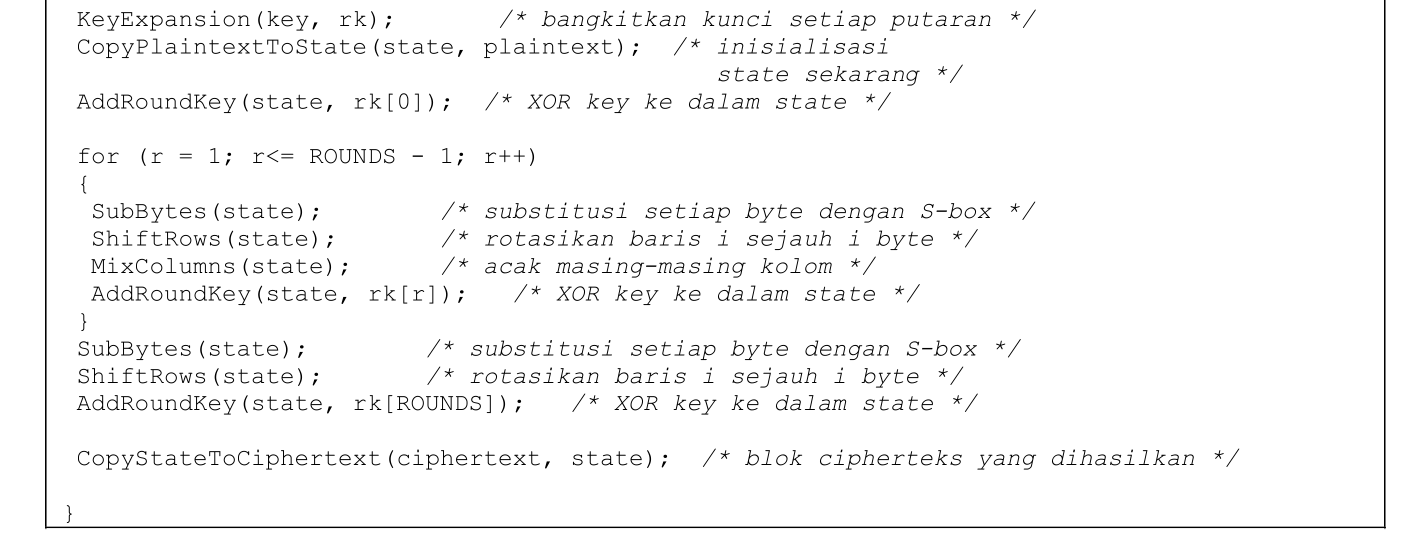
\includegraphics[width=153.51mm,height=151.77mm]{../../images/llm/page_014_img_01.png}%
\end{textblock*}

\end{document}
